\PassOptionsToPackage{quiet}{xeCJK}
\documentclass[withoutpreface,bwprint]{format}
\usepackage{ctex,etoolbox,mdframed,url,array,tabularx,longtable,booktabs,float}
\newcolumntype{C}{>{\centering\arraybackslash}X}
\newcolumntype{L}{>{\raggedright\arraybackslash}X}
\renewcommand{\textbf}[1]{{\song\bfseries #1}}
\usepackage{fancyhdr}
\pagestyle{fancy}\fancyhf{}\fancyfoot[C]{\zihao{-5}\thepage}
\renewcommand{\headrulewidth}{0pt}\renewcommand{\footrulewidth}{0pt}
\begin{document}
{\centering\zihao{3}\bfseries NIPT检测时点优化与异常标记判定模型\par}
\begin{abstract}
无创产前基因检测（NIPT）需要同时处理重复检测、达标概率、检测时点和异常标记判定。本文以附件中的男胎、女胎记录为对象，以孕妇代码为分组单位，建立可复现的主体层级建模框架。

\textbf{对于问题一，}在Y染色体浓度的logit尺度上建立随机截距线性混合模型，并以加性样条作非线性对照。孕周系数为0.04701，BMI系数为$-0.02446$，组内相关系数为0.7283；按孕妇留出的预测$R^2=-0.0302$，故将结果解释为群体关联而非个体预测承诺。

\textbf{对于问题二，}以Y浓度是否达到4\%建立边际二项概率模型，并将失败风险和延迟代价结合为条件风险。动态规划在连续BMI上联合确定分组和检测时点。中延迟M情景给出11周、11周6天、12周6天的三组方案，对应样本人数为200、25、42。

\textbf{对于问题三，}加入年龄、身高及孕产代理变量后，基础扩展模型Brier为0.11192，较Q2高0.00032，未显示稳定增益；因此保留问题二的简洁主线，并将多因素方案作为条件扩展。

\textbf{对于问题四，}对T13、T18、T21及任一异常标记分别拟合主体隔离的L2正则化Logistic模型。总体异常标记的AP为0.3823、Brier为0.08419。除MCC阈值外，设置训练层90\%灵敏度约束的漏诊优先方案；其外层总体灵敏度为0.8955、特异度为0.4033，展示漏诊与误报的权衡。

本文形成“重复测量解释—概率预测—风险决策—异常判定”的框架。结论仅适用于本附件、所列阈值与风险权重，不能替代临床确诊或独立队列验证。
\keywords{NIPT；线性混合模型；主体隔离验证；动态规划；Logistic回归}
\end{abstract}

\section{引言}
NIPT以母体外周血游离DNA为信息来源。男胎中，Y染色体浓度不足可能导致结果不可报告；女胎中，异常标记判定面对类别不平衡与少数阳性样本。附件中同一孕妇常有多次检测，故不能将每一行默认为独立样本。本文解决四项任务：解释Y浓度的纵向关联；在风险条件下确定BMI分组与时点；判断多因素能否稳定改善该决策；以及在检测后特征条件下判定女胎异常标记。

\section{总体分析}
四问按信息可得性的时间顺序递进：问题一以男胎Y浓度为连续响应，建立含孕妇随机截距的纵向模型；问题二将浓度转化为达标事件，对新孕妇预测边际概率并作风险优化；问题三比较多因素扩展的主体留出表现；问题四使用检测后可得的测序特征做异常标记判定。所有性能评价按孕妇划分训练、测试，折外记录不参与填补、标准化、拟合或阈值选择。

\section{模型假设}
\begin{itemize}[itemindent=2em]
\item 预约决策仅使用预约前或首条记录可得的信息，检测后质量变量不进入预约模型。
\item 同一孕妇的未观测稳定差异由随机截距刻画，给定固定效应和随机效应后残差近似独立。
\item 4\%为主分析浓度阈值，3.5\%和4.5\%只用于敏感性分析；搜索孕周为11至25周。
\item 问题四的异常标签为附件标记，供模型比较，不等同于临床确诊结局。
\end{itemize}

\section{符号说明}
\begin{longtable}{>{\centering\arraybackslash}p{0.20\textwidth}>{\centering\arraybackslash}p{0.72\textwidth}}
\caption{主要符号说明}\label{tab:symbol}\\\toprule
符号&含义\\\midrule\endfirsthead\toprule 符号&含义\\\midrule\endhead\bottomrule\endfoot
$Y_{ij}$&第$i$名孕妇第$j$次检测的Y染色体浓度\\
$g_{ij}$&检测孕周\\
$b_i$&孕妇$i$的随机截距\\
$p(t\mid x)$&特征$x$下孕周$t$达到浓度阈值的边际概率\\
$R(t\mid x)$&在孕周$t$检测的条件风险\\
$\lambda,\delta$&每周延迟代价与13周起附加代价\\
$q_i,h$&女胎异常预测概率与分类阈值\\
\end{longtable}

\section{模型的建立与求解}
\subsection{问题一：Y染色体浓度的重复测量模型}
男胎数据含267名孕妇、647条记录。将浓度比例作logit变换，主模型为
\begin{equation}
z_{ij}=\beta_0+\beta_1g_{ij}+\beta_2\mathrm{BMI}_{ij}+\beta_3g_{ij}\mathrm{BMI}_{ij}+b_i+\varepsilon_{ij},\quad b_i\sim N(0,\sigma_b^2).
\label{eq:lmm}
\end{equation}
孕周系数为0.04701、BMI系数为$-0.02446$，交互项没有稳定证据。组内相关系数0.7283表明主体层级不可省略。以孕妇为组作五折外层验证，主模型$R^2=-0.0302$；因此显著关联不被解释为对新个体的精确预测。
\begin{figure}[H]\centering

\includegraphics[width=.78\textwidth]{figures/result_q1_effect_bmi.png}
\caption{BMI对Y染色体浓度的边际影响}\label{fig:q1effect}
\end{figure}

\subsection{问题二：达标概率、风险函数与BMI分组}
定义达标事件$A_{ij}=I(Y_{ij}\geq0.04)$，在logit连接下拟合随机截距二项模型。对新孕妇积分随机效应，得到边际达标概率：
\begin{equation}
p(t\mid x)=\int \operatorname{logit}^{-1}\{\eta(t,x)+b\}\phi(b;0,\sigma_b^2)\,db.
\label{eq:prob}
\end{equation}
其中$x$为BMI。对每日网格孕周计算条件风险
\begin{equation}
R(t\mid x)=1-p(t\mid x)+\lambda(t-11)+\delta I(t\geq13).
\label{eq:risk}
\end{equation}
低延迟L、中延迟M、高延迟H分别取$(\lambda,\delta)=(0.005,0.10)$、$(0.020,0.10)$、$(0.050,0.10)$。本文选择M作为主答案：它同时保留失败和等待代价，避免L情景频繁出现25周边界解，也避免H情景将方案推向11周边界。

对BMI排序后，以动态规划最小化组内加权风险，约束最小组样本量、相同BMI不拆分和局部观测支持。表\ref{tab:q2policy}给出4\%阈值、M情景的有效三组解；边界显示到一位小数，优化使用未舍入值。
\begin{table}[H]\centering\small
\caption{问题二：4\%阈值、中延迟M情景下的条件方案}\label{tab:q2policy}
\begin{tabular}{cccc}\toprule BMI区间（kg/m$^2$）&人数&推荐检测时点&说明\\\midrule
$[20.7,33.4)$&200&11周&搜索域下界\\
$[33.4,34.4)$&25&11周6天&满足最小组样本量\\
$[34.4,46.9]$&42&12周6天&13周阶跃之前\\
\bottomrule\end{tabular}\end{table}
\begin{figure}[H]\centering

\includegraphics[width=.82\textwidth]{figures/result_q2_probability_surface.png}
\caption{不同孕周与BMI下的边际达标概率}\label{fig:q2surface}
\end{figure}

\subsection{问题三：多因素扩展与条件方案}
基础扩展规格加入首条记录年龄、身高；完整规格再加入辅助受孕、孕次与产次代理。原体重、身高和BMI不同时输入基础规格，检测后质量变量不进入预约模型。三种规格采用相同主体五折划分，以每名孕妇的外层Brier损失作配对比较，见表\ref{tab:q3compare}。
\begin{table}[H]\centering\small
\caption{多因素固定规格相对Q2的主体留出表现}\label{tab:q3compare}
\begin{tabular}{lccc}\toprule 规格&主体Brier&相对Q2差值&差值95\%区间\\\midrule
Q2：孕周与BMI&0.11160&0&--\\
基础扩展：加入年龄、身高&0.11192&0.00032&$[-0.00247,0.00312]$\\
完整扩展：再加孕产代理&0.11384&0.00224&$[-0.00132,0.00596]$\\
\bottomrule\end{tabular}\end{table}
两种扩展均未显示稳定改善。基础扩展在M情景下仍按BMI分组，得到$[20.7,33.4)$、$[33.4,35.0)$、$[35.0,46.9]$三组，推荐时点依次为11周、12周2天、12周6天；它是条件扩展结果，不替代问题二的主方案。

\subsection{问题四：女胎异常标记概率判定}
以T13、T18、T21及任一异常标记为四个二元目标，输入染色体Z值、X浓度、GC、读段与比对质量、孕周、BMI、年龄等14项检测后特征。对每个目标拟合L2正则化Logistic模型：
\begin{equation}
q_i=\frac{1}{1+\exp[-(\alpha_0+\alpha^Tv_i)]},\qquad \widehat A_i=I(q_i\geq h).
\label{eq:logit}
\end{equation}
采用三折分层主体外层验证；预处理、拟合和阈值选择均限制在训练主体内。MCC阈值在内层主体预测上选择。另设高灵敏度方案：在训练层选择灵敏度至少90\%的最高阈值，再由外层测试其可推广性。

总体异常标记的AP为0.3823、Brier为0.08419、ROC-AUC为0.7711。MCC阈值下总体灵敏度0.1791、特异度0.9851；高灵敏度方案的外层灵敏度0.8955、特异度0.4033。表\ref{tab:q4high}表明以大量假阳性换取较低漏诊风险，且T21仅有12名阳性主体，不能作临床高敏筛查承诺。
\begin{table}[H]\centering\small
\caption{高灵敏度约束阈值的主体隔离外层结果}\label{tab:q4high}
\begin{tabular}{lrrrrrr}\toprule 目标&阈值中位数&灵敏度&特异度&TP&FP&FN\\\midrule
T13&0.0199&0.9130&0.2612&21&430&2\\
T18&0.0605&0.8478&0.6315&39&206&7\\
T21&0.0058&0.8462&0.0726&11&549&2\\
任一异常&0.0562&0.8955&0.4033&60&321&7\\
\bottomrule\end{tabular}\end{table}

\subsection{结果解释与时点决策}
问题一中，随机效应引入的主体内相关性表明，常规逐行回归会错误放大有效样本量。图\ref{fig:q1comp}比较线性混合模型和样条对照的外层表现：两者均未得到正的主体留出$R^2$，因此选择线性混合模型作为关联解释的主模型，而不以复杂曲线追求表面拟合度。
\begin{figure}[H]\centering
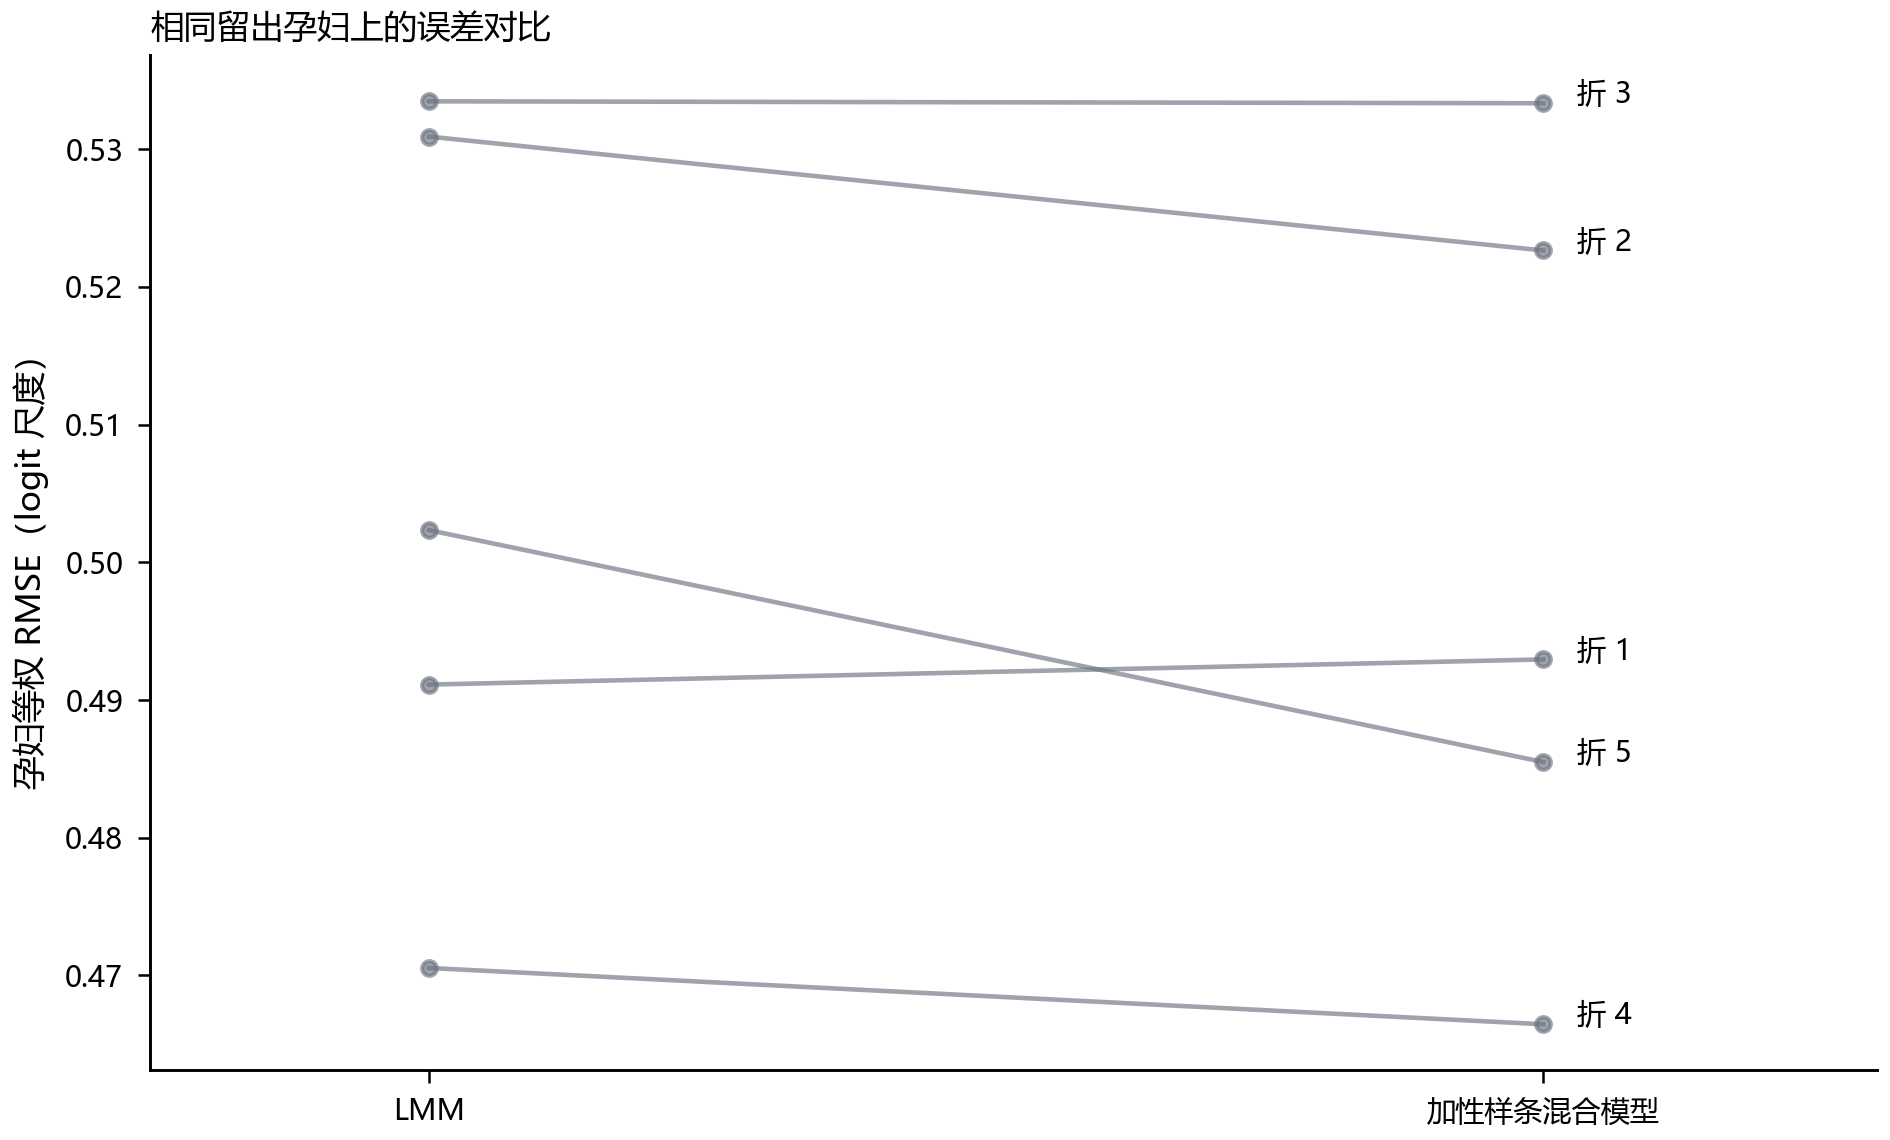
\includegraphics[width=.78\textwidth]{figures/result_q1_comparison.png}
\caption{问题一模型在主体留出验证中的比较}\label{fig:q1comp}
\end{figure}

问题二的三组时点来自达标概率、风险权重和支持约束的共同作用，而非BMI本身的临床分类边界。图\ref{fig:q2cal}显示主体留出概率校准情况；早孕及高BMI区域的支持较少，故策略不会在缺乏观测支持的区域作无约束外推。对不同风险权重，L情景更重视等待、但会在部分组产生25周边界解；H情景更重视延迟、因而倾向于11周边界。M情景位于两者之间，故用于主答案。
\begin{figure}[H]\centering
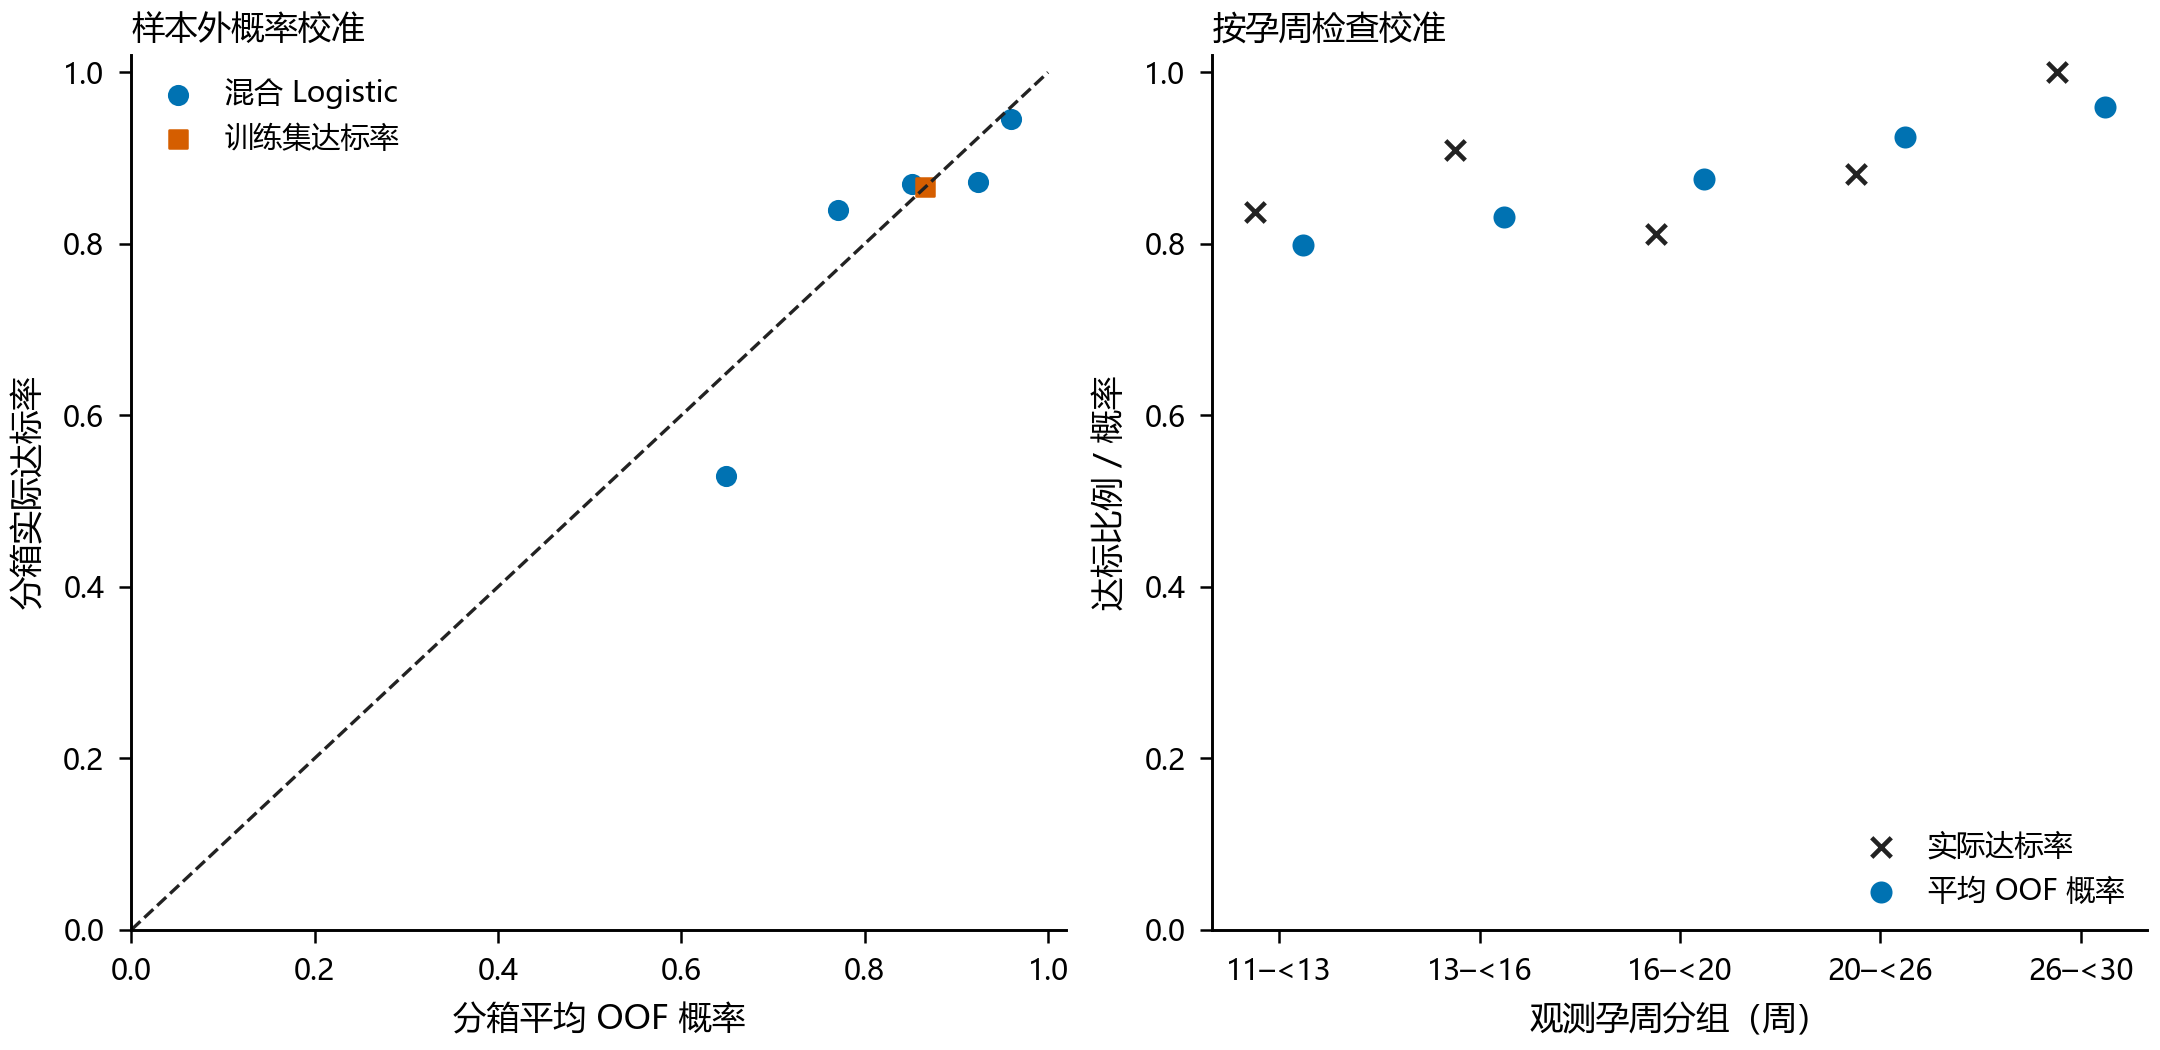
\includegraphics[width=.74\textwidth]{figures/process_q2_calibration.png}
\caption{问题二边际达标概率的主体留出校准}\label{fig:q2cal}
\end{figure}

问题三的扩展模型将个人年龄、身高代入概率后仍只按BMI排序分组，并在组内对实际协变量分布的风险求和；这避免把所有人固定为平均年龄和身高。图\ref{fig:q3policy}展示M情景下的扩展条件解以及L/M/H场景下的变化。由于表\ref{tab:q3compare}的配对区间跨过零，正文不把它解释成对Q2的优越替代。
\begin{figure}[H]\centering
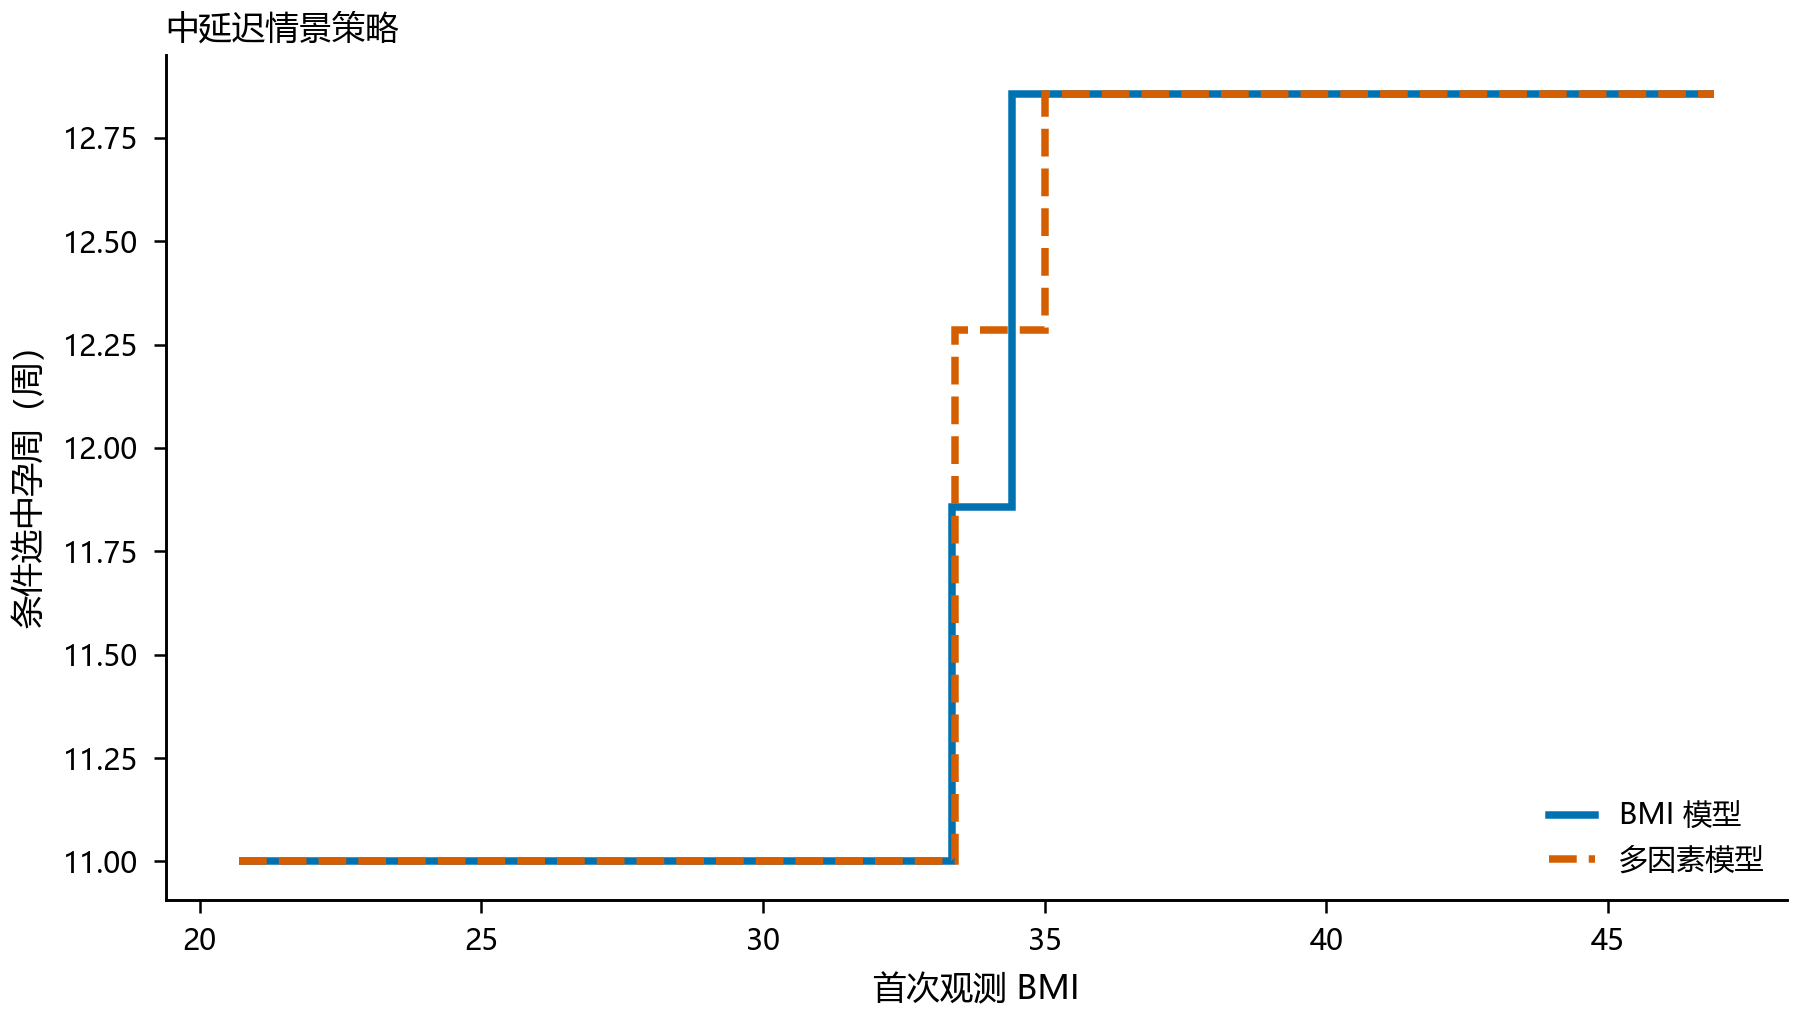
\includegraphics[width=.80\textwidth]{figures/result_q3_conditional_policy.png}
\caption{问题三多因素扩展下的BMI条件时点}\label{fig:q3policy}
\end{figure}

\subsection{问题四的判定口径}
异常类比例低时，准确率可由预测全部正常而虚高，因此同时报告ROC-AUC、AP、Brier、灵敏度、特异度与混淆矩阵。Brier分数定义为
\begin{equation}
\operatorname{Brier}=\frac{1}{N}\sum_{i=1}^{N}(q_i-A_i)^2.
\label{eq:brier}
\end{equation}
对固定的外层预测，先在每名孕妇内平均损失，再跨主体作2000次重采样。T18相对常数率的主体Brier差值为$-0.00929$，区间为$[-0.01685,-0.00294]$；任一异常标记的差值为$-0.01527$，区间为$[-0.02575,-0.00663]$。T13和T21区间均跨过零，不能宣称稳定增益。
\begin{figure}[H]\centering
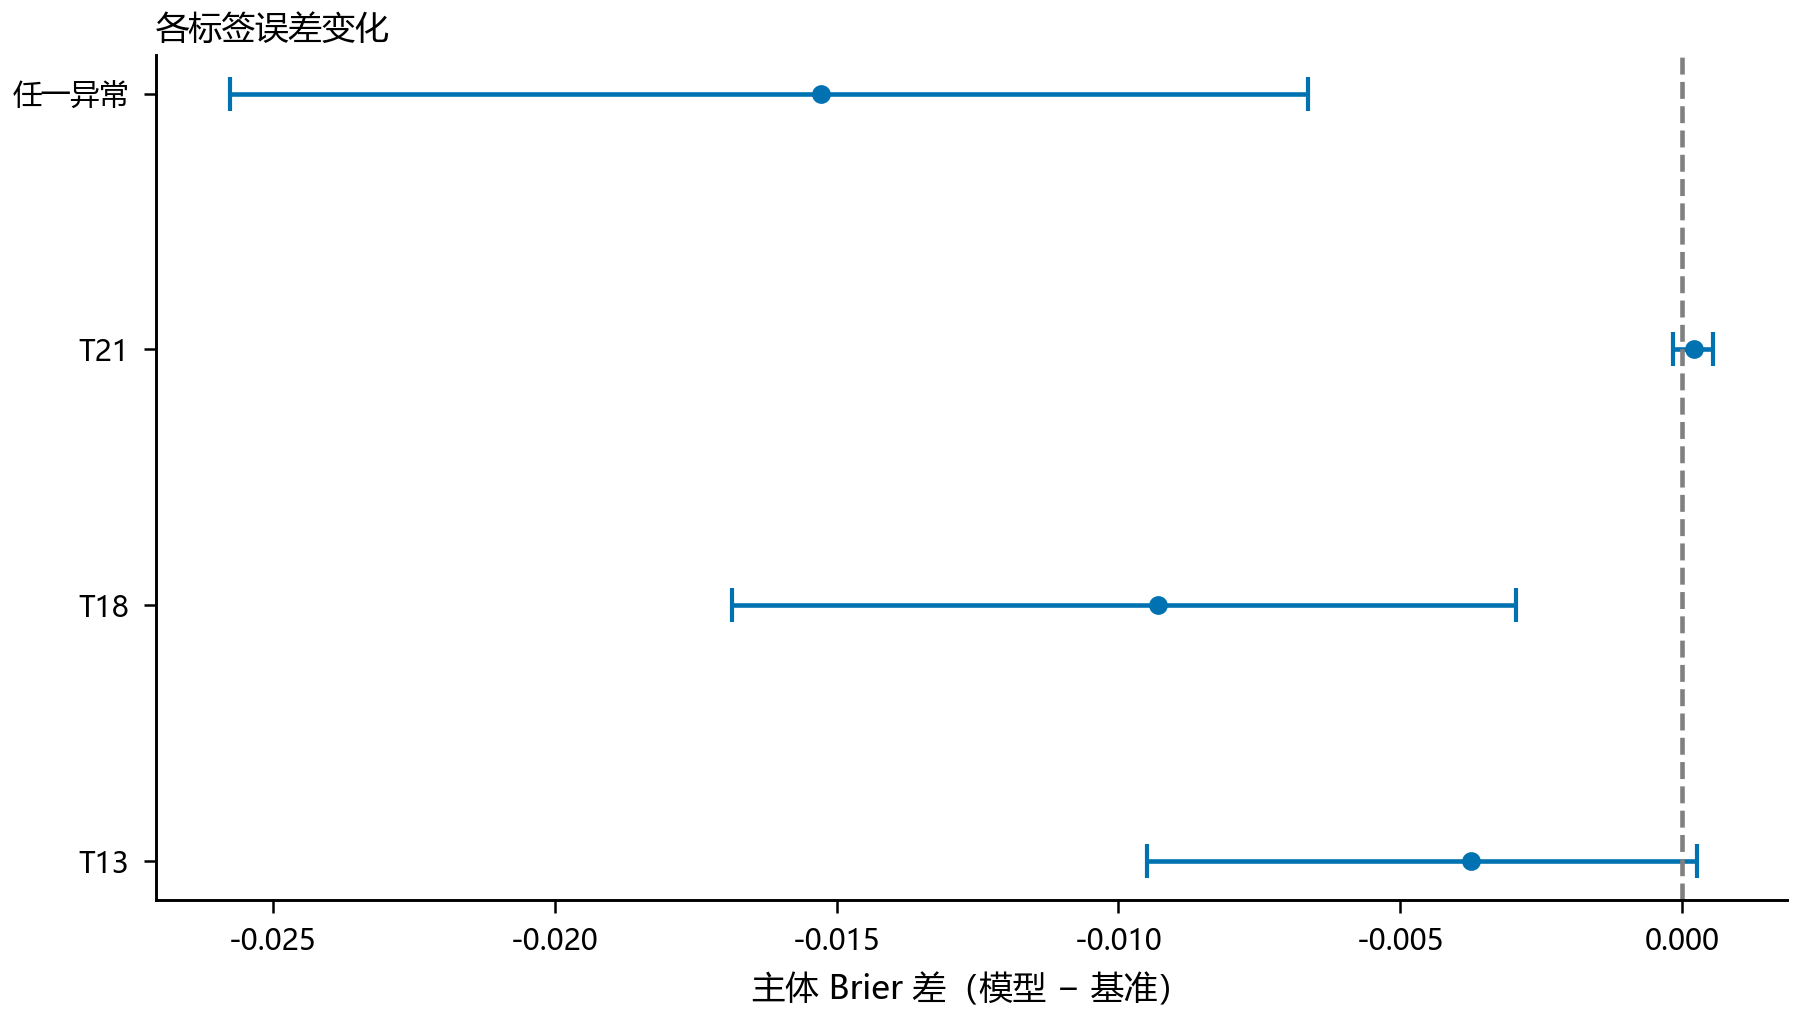
\includegraphics[width=.76\textwidth]{figures/result_q4_brier_intervals.png}
\caption{女胎各目标相对常数率的主体Brier差值区间}\label{fig:q4brier}
\end{figure}

\section{模型检验与分析}
\subsection{主体隔离验证}
问题一的负外层$R^2$说明关联与预测应分开表述。问题二检验概率校准，问题三以同折损失差值比较，问题四使用嵌套主体隔离阈值选择。由此避免了同一孕妇的相似记录同时出现于训练集和测试集造成的性能高估。

\subsection{阈值、风险与测量敏感性}
同次抽血重复测序组给出logit浓度波动尺度$\hat\sigma_m=0.123745$。按孕妇2000次重采样的区间约为$[0.08175,0.16770]$。在20轮主体重采样及四档追加噪声下重新拟合和优化，策略随样本构成而变化，故BMI切点只代表本附件、当前代价下的条件分割。
\begin{table}[H]\centering\small
\caption{Q2低延迟L情景的阈值敏感性}\label{tab:threshold}
\begin{tabular}{ccccc}\toprule 浓度阈值&有效组数&内部BMI切点&检测时点&对应人数\\\midrule
3.5\%&1&无&12周6天&267\\
4.0\%&2&33.8&12周6天；25周&212；55\\
4.5\%&2&29.1&12周6天；25周&38；229\\
\bottomrule\end{tabular}\end{table}
\begin{table}[H]\centering\small
\caption{女胎主体隔离外层记录级指标（MCC阈值）}\label{tab:q4metrics}
\begin{tabular}{lrrrrr}\toprule 目标&ROC-AUC&AP&Brier&灵敏度&特异度\\\midrule
T13&0.6796&0.1967&0.03317&0.1739&0.9210\\
T18&0.7943&0.2924&0.06252&0.5000&0.8551\\
T21&0.4467&0.0302&0.02123&0.1538&0.8361\\
任一异常&0.7711&0.3823&0.08419&0.1791&0.9851\\
\bottomrule\end{tabular}\end{table}

\section{模型的评价}
模型将孕妇、抽血和测序记录分层，避免重复记录造成虚假的独立样本量；将浓度关联、达标概率和风险优化拆开，使每个推荐时点可追溯至阈值、权重及可行性约束；且预处理和阈值选择均在训练主体内完成。局限是风险权重未由真实临床效用标定，早孕、高BMI及稀有异常覆盖有限，异常标签也非确诊金标准。高灵敏度阈值必须以独立阳性队列重新验证。

\section{模型的改进与推广}
补充预约前基线信息、早孕独立队列、复检成本和确诊结局后，可在不改变主体层级验证与风险优化框架的前提下重新标定概率与代价。该方法可推广至复检预约、连续生理指标随访和筛查流程优化；推广时必须重新定义可用信息、事件阈值、主体单位和风险权重，不能直接移植本题BMI切点或分类阈值。

\begin{thebibliography}{99}
\bibitem{wang2013} Wang E, Batey A, Struble C, et al. Gestational age and maternal weight effects on fetal cell-free DNA in maternal plasma. \textit{Prenatal Diagnosis}, 2013, 33(7): 662--666.
\bibitem{laird1982} Laird N M, Ware J H. Random-effects models for longitudinal data. \textit{Biometrics}, 1982, 38(4): 963--974.
\bibitem{yang2018} Yang J, Ding X, Zhu W. Improving the calling of non-invasive prenatal testing on 13-/18-/21-trisomy by support vector machine discrimination. \textit{PLOS ONE}, 2018, 13(12): e0207840.
\bibitem{efron1979} Efron B. Bootstrap methods: Another look at the jackknife. \textit{The Annals of Statistics}, 1979, 7(1): 1--26.
\end{thebibliography}

\makeatletter\let\@oldaddcontentsline\addcontentsline\renewcommand{\addcontentsline}[3]{}\section*{附录}\let\addcontentsline\@oldaddcontentsline\makeatother
\begin{table}[H]\centering\small
\caption{论文支撑材料及可复现入口}\label{tab:appendix}
\begin{tabularx}{\textwidth}{LX}\toprule 文件&说明\\\midrule
\texttt{src/run\_paper\_evidence.py}&一键重建数值证据、图表和测试\\
\texttt{src/q1\_lmm\_baseline.py}&问题一随机截距线性混合模型\\
\texttt{src/q2\_probability.py}&问题二边际达标概率和动态规划策略\\
\texttt{src/q4\_chromosomes.py}&问题四主体隔离Logistic及高灵敏度阈值\\
\texttt{outputs/}&模型输出、图表、指标与高灵敏度结果\\
\bottomrule\end{tabularx}\end{table}
\end{document}
